\section{Implementation details}
\label{sec:impl_details}

\begin{figure}
	\centering
	
	\begin{minipage}{0.435\linewidth}
		\includegraphics[width=\linewidth]{details/oxf_exs/ex1}
		
		\includegraphics[width=\linewidth]{details/oxf_exs/ex2}
		
		\includegraphics[width=\linewidth]{details/oxf_exs/ex4}
		
		\includegraphics[width=\linewidth]{details/oxf_exs/ex6}
		
		\includegraphics[width=\linewidth]{details/oxf_exs/ex3}
		
		\includegraphics[width=\linewidth]{details/oxf_exs/ex5}
		
		\scriptsize
		\begin{tabularx}
		{\linewidth}{X X X X}
			Reference images & 	Long-term & Snow queries & Night queries
		\end{tabularx}
	\end{minipage}\hfill	
	\begin{minipage}{0.555\linewidth}
		\includegraphics[width=\linewidth]{details/cmu_exs/ex1}
		
		\includegraphics[width=\linewidth]{details/cmu_exs/ex6}
		
		\includegraphics[width=\linewidth]{details/cmu_exs/ex4}	
		
		\includegraphics[width=\linewidth]{details/cmu_exs/ex2}	
		
		\includegraphics[width=\linewidth]{details/cmu_exs/ex3}	
		
		\includegraphics[width=\linewidth]{details/cmu_exs/ex5}	
		
		\scriptsize
		\begin{tabularx}{\linewidth}{X X X X}
			Reference images & Snow queries & Autumn queries & Long-term queries 
		\end{tabularx}
	\end{minipage}

	\caption[Examples of test images]{\label{fig:dataset} \textbf{Examples of test images :} we evaluate our proposal on 6 challenging localization sequences. Query image samples and the closest reference images in the database are presented from Oxford Robotcar~\cite{Maddern2016} (left) and CMU season dataset~\cite{Bansal2014a} (right).}
	
\end{figure}


\subsection{Dataset}
\label{subsec:dataset}
	We have tested our new method on the \textit{Oxford Robotcar} public dataset~\cite{Maddern2016} and the \textit{CMU Visual localization} dataset~\cite{Bansal2014a} from the city of Pittsburg. There are common dataset used for image-based localization~\cite{Sattler2018} and loop closure algorithm involving neural networks training~\cite{Porav2018} under challenging conditions.
		
\subsubsection{Training data}
	We use the temporal redundancy present in Oxford Robotcar dataset to build the images triplets to train our CNN. We build 400 triplets using three runs acquired at dates: \texttt{2015-05-19, 2015-08-28} and \texttt{2015-11-10}. We selected an area of the city different from the one used for training our networks for validation.
	Depth modality is extracted from the lidar point cloud. When re-projected in the image frame coordinate, it produces a sparse depth map. Since deep convolutional neural networks require dense data as input, we pre-process these sparse modality maps with inpainting algorithm from~\cite{Bevilacqua2017} in order to make them dense. We drop depth values larger than 100 meters in order to produce depth map with value in $[0, 1]$, consistent with the sigmoid decoder output.

\subsubsection{Testing data}
We propose six testing scenarios, 3 on each datasets. For the Oxford Robotcar dataset, the reference dataset is composed of 1688 images taken every 5 meters along a path of 2 km, when the weather was overcast. The three query sets are:
\begin{itemize}
	\item {Oxford -- Long-term (LT):} queries have been acquired 7 months after the reference images under similar weather conditions,
	\item {Oxford -- Snow:} queries have been acquired during a snowy day,
	\item {Oxford -- Night:} queries have been acquired at night, resulting in radical visual changes compared to the reference images.
\end{itemize}

For the CMU Visual localization dataset, the reference dataset is composed of 1944 images with a sunny weather and the three query sets are:
\begin{itemize}
	\item {CMU -- Long-term (LT):} queries have been acquired 10 months after the reference images under similar weather conditions,
	\item {CMU -- Snow:} queries have been acquired during a snowy day,
	\item {CMU -- Autumn:} queries have been acquired during Autumn, featuring warm-coloured foliage and low sunlight compare to the reference data.
\end{itemize}

\noindent Query examples are presented in figure~\ref{fig:dataset}.
	
\subsubsection{Evaluation metric}
for a given query, the reference images are ranked according to the cosine similarity score computed over their descriptors. To evaluate the localization performances, we consider two evaluation metrics:
\begin{itemize}
	\item \textbf{Recall @N:} we plot the percentage of well localized queries regarding the number $N$ of returned candidates. A query is considered well localized if one of the top $N$ retrieved images lies inside the $25m$ radius of the ground truth query position.
	\item \textbf{Top-1 recall @D:} we compute the distance between the top ranked returned database image position and the query ground truth position, and report the percentage of queries located under a threshold $D$ (from 15 to 50 meters), like in~\cite{Zamir2014}. This metric qualifies the accuracy of the localization system.
\end{itemize}


\subsection{Implementation}
\label{subsec:implementation}

Our proposal is implemented by using Pytorch as deep learning framework, ADAM stochastic gradient descent algorithm for the CNN training with learning rate set to 1e-4, weight decay to 1e-3 and $\lambda$ in triplet loss equal to 0.1. We use batch size between 10 and 25 triplets depending of the size of the system to train, convergence occurs rapidly and takes around 30 to 50 epochs. We perform both positive and negative hard mining, as in~\cite{Radenovic2017}. Images and depth maps are re-sized to $224\times224$ pixels before training and testing.

\subsubsection{Encoder architectures} 
We test the fully convolutional part of Alexnet and Resnet18 architectures for features extraction. As sown in~\cite{Piasco2019a}, we use the truncated version of Resnet18 to increase the spatial resolution of the final features block. Weights are initialized with the pre-trained weights on ImageNet. We always use Alexnet encoder to extract features from raw depth map, reconstructed depth map, or hallucinated depth map. Indeed the quality of our depth map is usually very low, we have found that using deeper network does not significantly improve localization results. We transform the 1-channel depth map into 3-channels jet colorization depth map in order to benefit from the convolutional filters learned on ImageNet. We do not use the 3-channels HHA depth map representation introduced in~\cite{Gupta2014} as it have been shown to perform equivalently to jet colorization~\cite{Eitel2015}.

\subsubsection{Descriptor architectures}
We test the two state-of-the-art image descriptors MAC~\cite{Radenovic2017} and NetVLAD~\cite{Arandjelovic2017}. MAC is a simple global pooling method that takes the maximum of each feature map from the encoder output. NetVLAD is a trainable pooling layer that mimics VLAD aggregation method. For all the experiments, we set the number of NetVLAD clusters to 64. Finally, both MAC and NetVLAD descriptors are $L_{2}$ normalized.

By combining Alexnet or Resnet encoder with MAC or NetVLAD descriptor pooling, we obtain 4 global image descriptor variants.

\subsubsection{Decoder architecture}
The decoder used in our proposal is based on Unet architecture and inspired by network generator from~\cite{Isola2017}. Dimension up-sampling is performed through inverse-convolutions layers. Decoder weights are initialized randomly.

\subsection{Competitors}
\label{subsec:competitors}
We compare the three following global image descriptors:
\begin{enumerate}
    \item \textit{RGB only (\textbf{RGB}):} simple networks composed of encoder + descriptor trained with only images, without side depth maps information. Networks are trained on Robotcar dataset following the standard procedure of image descriptor training with triplet loss~\cite{Arandjelovic2017, Radenovic2017}.
    \item \textit{Our proposal (\textbf{RGB(D)}):} network that use pairs of aligned image and depth map during training step and images only at test time. We follow training procedure as explained in~\ref{subsec:training}.
	\item \textit{Hallucination network (\textbf{RGB(H)}):} we compare our version of hallucination network~\cite{Hoffman2016}, trained on aligned triplets of images and depth maps. We follow training procedure of~\cite{Hoffman2016} to train the hallucination network.
\end{enumerate}

For fair comparison, as \textbf{RGB(D)} and \textbf{RGB(H)} image descriptors are obtain by concatenation two full-size descriptors (see section~\ref{subsec:fuse_desc}), we perform PCA to reduce the size of the final descriptor of all three methods to 2048.